\section{Evaluation}\label{sec:evaluation} 
In this chapter, I am going to evaluate the outcome of my thesis i.e. research and implementation work. 
Figure~\ref{fig:Evaluation_Phases} shows the phases of the entire evaluation process. Section \ref{subsec:goals} describes the research and case study phase. Section \ref{subsec:designmethod} illustrates the evaluation design method that I have used for conducting the experiment. This is then followed by a brief description of the planning phase in Section \ref{subsec:planning}. Afterward, Section \ref{subsec:investigationgoals} deals with the formulas to investigate the goals of the evaluation process. Then, Section \ref{subsec:execution} describes the preparation and test execution phase in detail. Section \ref{subsec:threats&mitigation} explains the associated threats with the evaluation process and their mitigation criteria. At last, Section \ref{subsec:results} discusses the result generated from the gathered data. 

The aim of this chapter is as follows: 

\textbf{"Analyse the outcome of the usage of an interactive demonstrator for the purpose of evaluation with respect to the user from the point of view of the researcher in the context of spreading the basic concepts of bidirectional transformation (bx) and making them understandable and accessible."}

\subsection{Goals}\label{subsec:goals}  
In any research, there could be many cases and each case could focus on a number of different research questions, each of which leads to a different direction in developing solution strategies~\cite{semethods}. Hence, for any evaluation process, most important thing are selecting cases that are most relevant to the research and narrowing down the research questions only associated with the exact problems in hand. 

\begin{figure}
	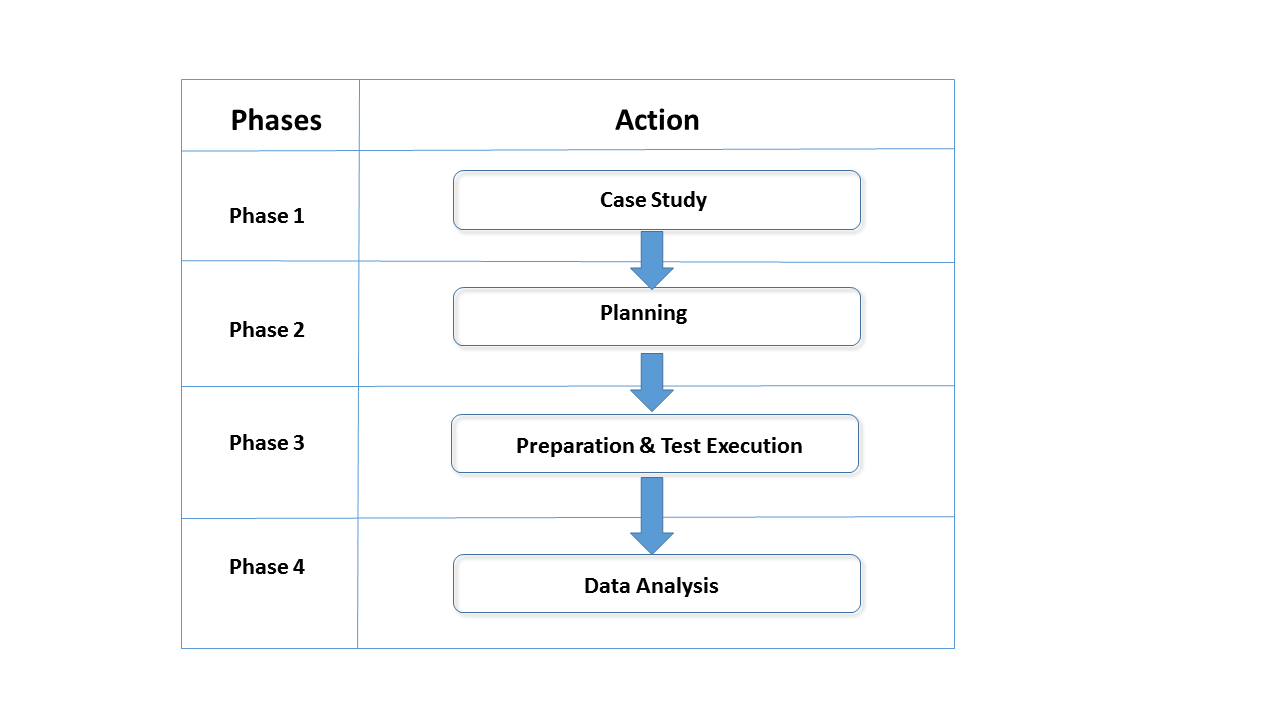
\includegraphics[width=1\textwidth]{figures/Evaluation_Phases}
	\caption{Evaluation Phases}
	\label{fig:Evaluation_Phases}
\end{figure}

\paragraph{Research Questions}
Our experience based on teaching and cooperation with industry has led us to suspect that people often draw their intuition for desired synchronization behavior directly from the special case of bijections.
This can be problematic and leads to statements such as: ``Why do I need a \emph{bidirectional} transformation language if the transformation at hand is not \emph{bijective}?''
Ironically, bidirectional transformation languages are often especially helpful when a transformation is \emph{not} bijective. As a sub-question of the research question \textbf{RQ 3} described earlier in Section \ref{subsec:contribution}, I propose to investigate if such misconceptions are really widespread or not:

\begin{description}
	\item[RQ 3.1:] Do people tend to derive their (in general wrong) intuition for synchronization scenarios from the special case of bijections?
\end{description}

To impart and train a more general intuition for synchronization scenarios I have implemented \texttt{Demon-BX}, an online demonstrator for bidirectional transformations, as a platform for easily creating synchronization scenarios to help achieve corresponding learning goals.
As a proof-of-concept, I have formulated five concrete learning goals and designed corresponding scenarios based on a simple example. We believe (i) that example-based demonstrators are an effective way of achieving my (and similar) learning goals, and (ii) that a demonstrator is only useful in combination with carefully designed scenarios. As a sub-question of the research question \textbf{RQ 4} described earlier in Section \ref{subsec:contribution}, I propose to investigate these conjectures with the following two research questions: 

\begin{description}
	\item[RQ 4.1:] Does demon-bx support achieving corresponding learning goals?
	\item[RQ 4.2:] How much does this support depend on the scenarios?  Would just playing with the demonstrator and the example already have an equal or comparable (positive) effect?
\end{description}

\paragraph{Purpose}
The purpose of the experiment is to evaluate whether it is possible to teach and enhance the understanding of the basic concepts of bx through the demonstrator.

\paragraph{Perspective}
The perspective is from the point of view of the researcher, i.e. the researcher would like to know if the usage of the demonstrator enhances the understanding of bx concepts of a user.

\paragraph{Context}
This experiment is on a bx tool demonstrator which falls under an educational environment and specifically under computer science branch. Hence, this experiment is mainly designed for the group of students/teachers/researchers from computer science area with or without prior knowledge of model driven software development field.

\subsection{Design Method}\label{subsec:designmethod} 
To investigate my research questions, I have used the Pretest-Posttest design method~\cite{analysisprepostdesigns}, a paired data analysis method in which the same experimental object is measured on some variables on two different occasions under different testing conditions. Here, I am using an extension of the Pretest-Posttest design method, called Pretest-Posttest control group design~\cite{expandquasiexpdesign}. It is a highly prestigious and one of the most popular research designs in use. The design principle is relatively simple, which involves two groups, a test group and a control group. First, the groups are pre-tested and then the test group is given the treatment. Afterward, both the groups are post-tested and data is collected from both occasions. Then, the analysis is done by comparing pretest and posttest results collected from both the groups as explained in Figure~\ref{fig:PrePost_Test}.

\begin{figure}
	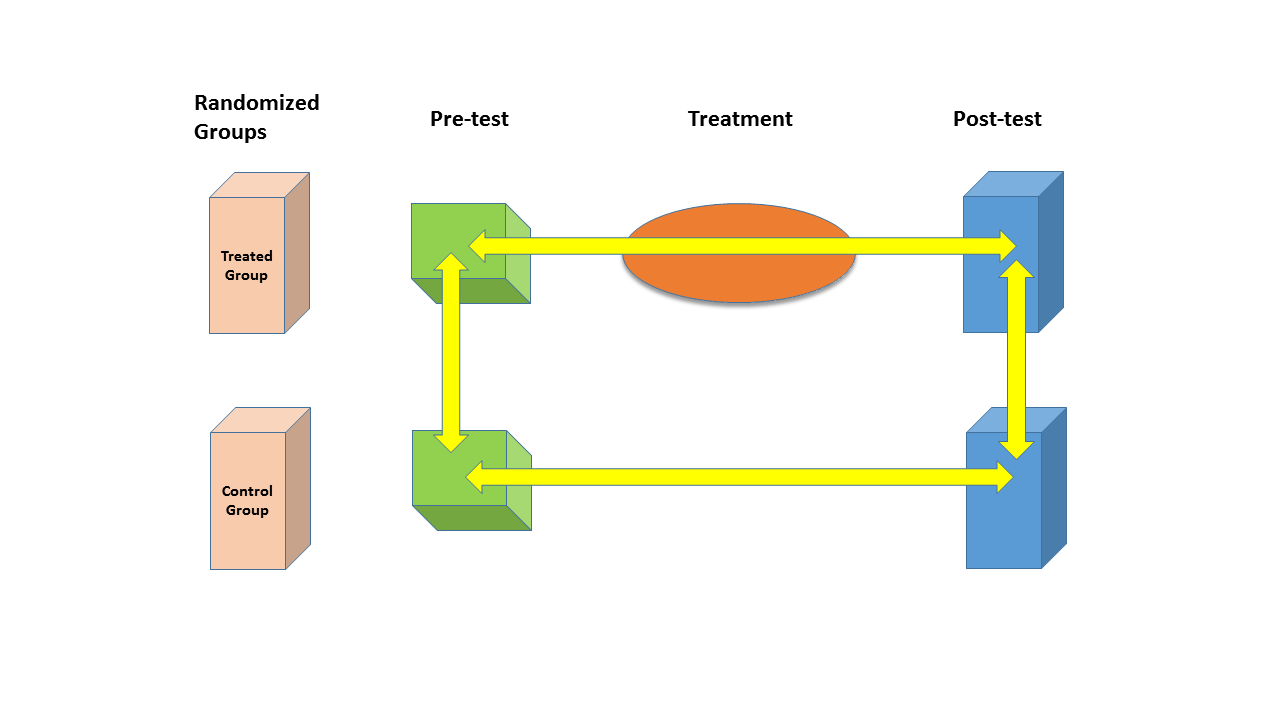
\includegraphics[width=1\textwidth]{figures/PrePost_Test}
	\caption{Pretest-Posttest Control Group Design }
	\label{fig:PrePost_Test}
\end{figure}

Selection of the Pretest-Posttest control group design method for the experiment is driven by the following reasons~\cite{anovapreposttest}:
\begin{itemize}
	\item It provides control over threats to internal validity.
	\item This allows the researchers to collect and compare posttest result from two groups, which give them an idea about the effectiveness of the treatment.
	\item The researcher can see how the groups have performed from pretest to posttest, whether one, both or neither improved over time.
\end{itemize}

In my case, I have designed test questions, one for each learning goal (brief description in Section~ \ref{subsubsec:questions}), to check if a participant has attained the learning goals or not.
We are also interested in the participants' subjective level of certainty for every given answer. 
The experiment is to be conducted as follows:

\begin{enumerate}
	\item All participants are divided randomly into two groups of equal size: the treated group and the control group.
	\item All participants take the pretest (answer all test questions).
	\item Both groups are allowed to use demon-bx for the same amount of time and are provided with an introduction and overview of the concrete example used in the demonstrator.
	The treated group is additionally provided with carefully chosen scenarios to work through, while the control group is not.
	\item When the time is up, all participants take the posttest (answer the same test questions again).
\end{enumerate}

\subsection{Planning}\label{subsec:planning}
This section explains the entire planning phase in detail. In this phase, I have investigated and  finalized all the factors required to evaluate the research questions as well as the execution of the experiment. Following sub-sections describe the factors one by one.

\subsubsection{Participants}\label{subsubsec:participants}
As the context of the experiment is mainly focussed only on the computer science area, it will be conducted on a group of masters' student of computer science branch at Paderborn University. The participants are chosen based on convenience, i.e. the participants are the students taking a similar course.

\subsubsection{Hypotheses}\label{subsubsec:hypotheses}
Formulating hypotheses formally state that what is going to be evaluated in the experiment. I have constructed my hypotheses focussing on the research questions \textbf{RQ 3.1}, \textbf{RQ 4.1}, and  \textbf{RQ 4.2} as described in Section \ref{subsec:goals}. Following are the hypotheses I have chosen to focus in my experiment:\\

\begin{description}
	\item[Operational Hypothesis]
	\item[H$_{OP1}$:] Students derive their (in general wrong) intuition for and expectations of synchronization scenarios from the special case of bijections.
	\item[H$_{OP2}$:] The use of demon-bx has a positive effect on the achievement of corresponding learning goals.\\
	\item[H$_{OP2}$:] The use of demon-bx in combination with suitable scenarios has a positive effect on the achievement of corresponding learning goals.\\
\end{description}

To evaluate the above stated hypotheses, the corresponding null hypotheses are stated below:
\begin{description}
	\item[Null Hypothesis]
	\item[H$_{NU1}$:] Students do not derive their (in general wrong) intuition for the synchronization scenarios.
	\item[H$_{NU2}$:] There is no significant improvement in the learning outcome of the students after using the demon-bx.
	\item[H$_{NU3}$:] There is no significant improvement in the learning outcome of the treated group compared to the control group.

\end{description}

\subsubsection{Experimental Variables}\label{subsubsec:expvariables}
Hypothesis described above helped in deciding the variables related to the experiment. Following paragraphs describe and Table~\ref{tab:Experimental_Variables} summarizes all of them .

\paragraph{Independent Variables} The independent variables, which the experimenter purposely changes during the experiment are listed below:

Does a group get scenarios to work through or not: nominal (yes or no)

\paragraph{Controlled Variables} The controlled variables, which are kept the same throughout the experiment are listed below:

Demonstrator platform: Demon-BX\\
Concrete example: Arranging a Kitchen\\
Group participants are chosen from: \{master students, PhD students, bx researchers, \ldots \}\\
Test questions: 5\\
Learning goals: 5\\
Max. time interval to answer questions: 55 min

\paragraph{Dependent Variables} The dependent variables, which are likely to be changed in response to the independent variable are listed below:

Correctness score of pretest: ordinal\\
Correctness score of posttest: ordinal\\
Level of certainty of pretest:  ordinal\\
Level of certainty of posttest: ordinal

\begin{table}
	\centering	
	\begin{tabular}{|p{4cm}|p{5cm}|p{6cm}|}
		\hline
		\rowcolor[gray]{.8}	
		\textbf{} & \textbf{Name} & \textbf{Possible Values} \\
		\hline
		Independent Variable & Group gets scenarios to work & nominal (yes or no)\\
		\hline
		Controlled Variables & 
		Demonstrator Platform 
		\newline Concrete Example
		\newline Group participants
		\newline Test questions
		\newline Learning goals
		\newline Max. time interval	&
		Demon-BX
		\newline Arranging a Kitchen 
		\newline \{master students, PhD students, \ldots \}
		\newline 5
		\newline 5
		\newline 55 min \\
		\hline	
		Dependent Variables & 
		Correctness score of pretest
		\newline Correctness score of posttest 
		\newline Level of certainty of pretest
		\newline Level of certainty of posttest & 
		ordinal
		\newline ordinal
		\newline ordinal
		\newline ordinal \\
		\hline				
		
	\end{tabular}
	\caption{Experimental Variables}
	\label{tab:Experimental_Variables}
\end{table}

\subsubsection{Learning Goals \& Questions}\label{subsubsec:questions}
To investigate the research questions \textbf{RQ 3} and its sub-question \textbf{RQ 3.1}, I carefully chose five bx concepts to evaluate and imply them as the learning goals (referred to as \textbf{LG} from now on) for the experiment. These concepts are related to the basic fundamentals of bx described as follows:
\begin{description}
	\item[LG 1:] It is possible to avoid/minimize unnecessary information loss in bx. 
	\item[LG 2:] Not all possible changes done in one model can be translated/synchronized into another model.
	\item[LG 3:] Synchronisation is interactive. User interaction (or some other, possibly automated means) can be used to decide between multiple equally consistent results (to handle non-determinism). 
	\item[LG 4:] Undoing changes in one model to revert to a previous state does not necessarily imply that this can be reflected analogously in the other model. 
	\item[LG 5:] Bx frameworks are not always state based but also can be delta based. The actual change performed can have an effect on synchronization results, even if the final result might appear to be exactly the same in both cases. 
\end{description}

To evaluate these learning goals, I prepared five questions. Each question referred to a concept of bx which also corresponds to a learning goal.

The questions are designed to have two sections for answers. One section contains multiple choice answers and the other contains certainty scale ranging from "I just guessed" to "I am certain". Correctness will be decided from the selection of answer in multiple choice section and certainty will be decided from the certainty parameters. Hence, combining the answer and the certainty parameter I can differentiate between \emph{correct answer}, \emph{absolute correct answer}, \emph{wrong answer}, and \emph{absolute wrong answer}.

\subsection{Execution}\label{subsec:execution} 
This section explains the entire experiment execution process in detail along with the preparation steps in the following subsections.

\subsubsection{Preparation }\label{subsubsec:prep}
To handle two separate groups i.e., control and treated and to conduct two separate tests i.e., pre-test and post-test on them, I had to prepare well before the experiment date. 

First, I prepared a two-minute video tutorial explaining some of the basic concepts of bx. Then, I prepared a set of questions  relating each question to one learning goals and put them into two different forms  i.e., pretest and posttest prepared with google forms to make them available online for the sake of easy sharing. Then to investigate the research questions \textbf{RQ 4} and its sub-question \textbf{RQ 4.1}, I prepared the scenarios with the demonstrator to explain the learning goals in a simple way but with a concrete example. Finally, I prepared two different instruction sheets for both the groups explaining the steps they need to follow during the experiment.

\subsubsection{Test Execution}\label{subsubsec:execution}
The experiment was performed on a group of Master students attending a computer science lecture at Paderborn University. They were informed in advance that such experiment will be conducted on a particular date and that their participation in the experiment is completely voluntary with no consequences what so ever. Participants were requested to bring their laptops to the lecture on the day of the experiment.

\paragraph{Confidentiality} The participants were informed regarding the confidentiality and anonymity of data. The purpose of evaluating the tool was stated, but not the hypotheses of the experiment.

\paragraph{Randomization} To perform the experiment, the students were given the instruction sheet prepared earlier for either the control or the treated group randomly while entering the room. The participants were not informed about which group they are in and received suitable and separate instructions for each group.

\paragraph{No Interference} After that, they were asked to sit in two different areas according to their group allotment. The groups were spatially separated so that discussion between groups was almost impossible.

These information sheets had all the appropriate links to the corresponding questionnaires with questions for the pre-test and post-test, demonstrator links with prepared scenarios for the treated group, and a different demonstrator link without scenarios for the control group.

Firstly, all participants went through a two-minute video tutorial to establish basic concepts and notation used in the test questions. Then all participants were asked to take the pre-test. After finishing the pre-test, the students were asked to use the demonstrator links given to them and to work with it. The link given to the control group only had information on how to operate the demonstrator, while the treated group had access to scenarios chosen to support my learning goals. 

After playing with the demonstrator, both groups were asked to take the post-test. Post-test questions were exactly the same as pre-test questions but include some extra questions to get additional qualitative feedback about the demonstrator. The experiment was stopped exactly after 55 minutes.

\subsubsection{Data Validation}\label{subsubsec:datavalidation}
Data was collected from 40 students. I stopped taking responses on Google forms i.e. pre-test and post-test forms from students exactly after 55 minutes. After the experiment, I checked the data entered by students in both the forms. Data from one student was removed, due to the fact that the data was regarded as invalid as the student could not finish both the test in the given time limit.

Hence, after removing one student out of the 40, I had data from 39 students for statistical analysis and interpretation of the results.

Finally, based on unique identifiers (identifying the group and participant uniquely) derived for each participant, answers from pre-test and post-test were evaluated to get the results. 

\subsection{Threats to Validity and Mitigation}\label{subsec:threats&mitigation}
A good research work depends highly on its validity and quality of work involved and results. So, it is very important to consider, analyze and mitigate the validity threats to the research work and the results. In my evaluation, I have focused on the validity analysis and threats given by Wohlin et al~\cite{expinse} and further explained by Feldt et al~\cite{validitythreatsinse}. Wohlin et al discuss four main types of validity threats: internal, external, construct and conclusion. 

This section describes all the threats that are associated with the entire evaluation process i.e., planning, preparation, and execution in the following subsections.
 
\subsubsection{Internal Validity}\label{subsubsec:internalvalidity}
\emph{Did the treatment/change I introduced cause the effect on the outcome? Can other factors also have had an effect?}

\medskip
\noindent To measure improvement I am forced to perform arithmetic with ordinal values.
This might be problematic as the difficulty of the test questions might not be equal (although I have tried to ensure this). If, for example, one of the test questions is much more difficult than all the rest, then subtracting test scores and comparing improvements between groups is questionable. Hence to make the questions/concepts more understandable, I have provided some explanations in the post-test as a video tutorial showing the relation between the abstract example and a concrete example.

\subsubsection{External Validity}\label{subsubsec:externalvalidity}
\emph{Is the cause and effect relationship I have shown valid in other situations?}

\medskip
\noindent Our results are only valid for the choice of control variables.
This can be problematic as, for example, my test questions might not actually be suitable for checking if my learning goals have been reached.

\subsubsection{Construct Validity}\label{subsubsec:constructvalidity}
\emph{Do the groups involved in the experiment equally balanced to have a positive effect on the outcome I measure?}

\medskip
\noindent It might be possible that students of equal caliber are sitting together or might have a discussion between the test to have a negetive effect on the results. Hence to avoid that, I have randomly selected students for control and treated group by giving them instruction sheets randomly while entering the class and making them sit in two separate groups apart from each other.

\subsubsection{Conclusion Validity}\label{subsubsec:conclusionvalidity}
\emph{Does the treatment/change I introduced have a statistically significant effect on the outcome I measure? Can I draw conclusions based on the data?}
	
\medskip
\noindent A problem could be that participants just guess the answers wildly. So it might possible that the data could be faked or incorrect due to mistakes. To avoid faking of data and to add more authenticity to the experiment, I have added certainty values for each question so that I will get to know whether the participant is just guessing the answer or certain about it. Also, I have scrambled the order of the scenarios given to the treated group to play with and the questions asked so that participants will not get a clue about the relation between them.

\subsection{Data Analysis, Results, and Discussion}\label{subsec:results}
To get the results for my experiment, I have investigated on each hypothesis with the data collected separately. Analysis of the data, descriptive statistics are used to visualize the data collected and described in the following subsections.

\subsubsection{Analyzing Hypothesis 1}\label{subsubsec:hypothesis1}
Hypothesis 1 i.e., \textbf{H$_{OP1}$} and \textbf{H$_{NU1}$} is designed to investigate research question \textbf{RQ 3.1}.
\paragraph{Formula} Data for \textbf{RQ 3.1} can be collected from all pretest results i.e., combining the pretest results from both control and treated group. As five questions were asked, result can be calculated for each question from the pretest data. 

Calculation of the result for each question involves the correctness and certainty of the answers given by the students.
For ith Question \textit{Q$_{i}$},

\textit{CO$_{pre(i)}$} $\epsilon$ \{-1, 1\}, correctness of the answer to the ith pretest question is either right (1) or wrong (-1).

\textit{CE$_{pre(i)}$} $\epsilon$ [0, 1], certainty of the answer to the ith pretest question is between 0 ("I just guessed") to 1 ("I am certain").

\textit{RES$_{pre(i)}$} := \textit{CO$_{pre(i)}$} * \textit{CE$_{pre(i)}$} $\epsilon$ [-1,  1], result for the ith pretest question is between -1 to 1.

For the final calculation, following result will be considered:\\
\textit{R$_{pre(i)}$}:= Set containing all the \textit{RES$_{pre(i)}$} calculated from the answers to the ith pretest question.

Null Hypothesis, {H$_{NU1}$}: Mean (\textit{R$_{pre(i)}$}) <= 0

Operational Hypothesis, {H$_{OP1}$}: Mean (\textit{R$_{pre(i)}$}) > 0

\paragraph{Data Analysis}
\paragraph{Discussion}

\subsubsection{Analyzing Hypothesis 2}\label{subsubsec:hypothesis2}
Hypothesis 2 i.e., \textbf{H$_{OP2}$} and \textbf{H$_{NU2}$} is designed to investigate research question \textbf{RQ 4.1}.

\paragraph{Formula}
Data for \textbf{RQ 4.1} can be collected from all pretest and posttest results i.e., combining the pretest results from both control and treated group and combining the posttest results from both control and treated group. As five questions were asked, result can be calculated for each question from the pretest and posttest data. 

Calculation of the result for each question involves calculation of improvement in correctness and certainty of the answers given by the students in posttest than pretest.
For ith Question \textit{Q$_{i}$},

\textit{CO$_{pre(i)}$} $\epsilon$ \{-1, 1\}, correctness of the answer to the ith pretest question is either right (1) or wrong (-1).

\textit{CE$_{pre(i)}$} $\epsilon$ [0, 1], certainty of the answer to the ith pretest question is between 0 ("I just guessed") to 1 ("I am certain").

\textit{RES$_{pre(i)}$} := \textit{CO$_{pre(i)}$} * \textit{CE$_{pre(i)}$} $\epsilon$ [-1,  1], result for the ith pretest question is between -1 to 1.

\textit{CO$_{post(i)}$} $\epsilon$ \{-1, 1\}, correctness of the answer to the ith posttest question is either right (1) or wrong (-1).

\textit{CE$_{post(i)}$} $\epsilon$ [0, 1], certainty of the answer to the ith posttest question is between 0 ("I just guessed") to 1 ("I am certain").

\textit{RES$_{post(i)}$} := \textit{CO$_{post(i)}$} * \textit{CE$_{post(i)}$} $\epsilon$ [-1,  1], result for the ith posttest question is between -1 to 1.

\textit{IMP$_{(i)}$} := (\textit{RES$_{post(i)}$} - \textit{RES$_{pre(i)}$})/2 $\epsilon$ [-1,  1], improvement for the ith question from pretest to posttest is between -1 to 1.

For the final calculation, following result will be considered:\\
\textit{I$_{(i)}$}:= Set containing all the \textit{IMP$_{(i)}$} calculated from the answers.

Null Hypothesis, {H$_{NU1}$}: Mean (\textit{I$_{(i)}$}) <= 0

Operational Hypothesis, {H$_{OP1}$}: Mean (\textit{I$_{(i)}$}) > 0

\paragraph{Data Analysis}
\paragraph{Discussion}
\subsubsection{Analyzing Hypothesis 3}\label{subsubsec:hypothesis3}
Hypothesis 3 i.e., \textbf{H$_{OP3}$} and \textbf{H$_{NU3}$} is designed to investigate research question \textbf{RQ 4.2}.

\paragraph{Formula}
Data for \textbf{RQ 4.2} can be collected from all pretest and posttest results separately from control and treated group. As five questions were asked, result can be calculated for each question from the pretest and posttest data separately for control and treated group. 

Calculation of the result for each question involves calculation of improvement in correctness and certainty of the answers given by the students in posttest than pretest separately for control and treated group.
For ith Question \textit{Q$_{i}$},

Parameters used in the below formulas e.g., \textit{RES$_{post(ci)}$}, \textit{RES$_{pre(ci)}$}, \textit{RES$_{post(ti)}$}, \textit{RES$_{pre(ti)}$} are calculated similar to the formulas as described in Section \ref{subsubsec:hypothesis2} but separately for control and treated group.

\textit{IMP$_{(ci)}$} := (\textit{RES$_{post(ci)}$} - \textit{RES$_{pre(ci)}$})/2 $\epsilon$ [-1,  1], improvement for the control group for the ith question from pretest to posttest is between -1 to 1.

\textit{IMP$_{(ti)}$} := (\textit{RES$_{post(ti)}$} - \textit{RES$_{pre(ti)}$})/2 $\epsilon$ [-1,  1], improvement for the treated group for the ith question from pretest to posttest is between -1 to 1.

For the final calculation, following result will be considered:\\
\textit{I$_{(ci)}$}:= Set containing all the \textit{IMP$_{(ci)}$} calculated from the answers of the control group.

\textit{I$_{(ti)}$}:= Set containing all the \textit{IMP$_{(ti)}$} calculated from the answers of the treated group.

Null Hypothesis, {H$_{NU1}$}: Mean (\textit{I$_{(ci)}$})  - Mean (\textit{I$_{(ti)}$}) < 0

Operational Hypothesis, {H$_{OP1}$}: Mean (\textit{I$_{(ci)}$})  - Mean (\textit{I$_{(ti)}$}) > 0


\paragraph{Data Analysis}
\paragraph{Discussion}